\documentclass[11pt]{book}
\usepackage{amsmath}
\usepackage{geometry}
\usepackage{epstopdf}
\usepackage{hyperref}

\usepackage{amssymb}
\usepackage{graphicx}
\usepackage{braket}
\usepackage{paralist}
\usepackage{eufrak}
\usepackage{amscd}

\title{Notes}
\author{Zhu Yong Ting}
\def\bE{{\mathbb{E}}}
\def\bR{{\mathbb{R}}}

\def\eqlaw{{\stackrel{\text{(law)}}{=}}}
\def\tS{{\widetilde{S}}}
\def\tB{{\widetilde{B}}}
\def\tmu{{\widetilde{\mu}}}
\def\tsigma{{\widetilde{\sigma}}}
\def\abs#1{{\left|#1\right|}}
\def\E{{\mathrm{E}\,}}
\def\EE#1{{{\mathrm{E}}\left(#1\right)}}


\def\tX{{\widetilde{X}}}
\def\tM{{\widetilde{M}}}
\def\tx{{\widetilde{x}}}
\def\tm{{\widetilde{m}}}


\usepackage{hyperref}

\usepackage{natbib}


\begin{document}
 \bibliographystyle{cje}

\maketitle
\chapter{introduction}


An {\it option} is a contract which gives the holder the right but not the obligation to buy or sell an underlying asset at or before a certain date at an agreed price, as mentioned in \citeauthor{Hull2008}.
To get this right, the buyer should pay the seller. The price set in the contract is known as the {\it strike price}; the date is known as {\it expiration date} or {\it maturity}. There are always two sides involved in every option contract. On one side is the investor who has bought the option. This side is known as the long position. Another side is the short position who has sold the option. A {\it call} option gives the holder the right to buy the underlying asset, while a {\it put} option gives the holder the right to sell the underlying asset. European options can be exercised only at the expiration date. American options on the other hand may be exercised at any time before the expiration date.

To help the understanding of option, here we can give an example of the use of an option. Suppose that it is now January 15. A copper fabricator expects it will need 100,000 pounds of copper on May 15 to meet a certain contract. The spot price of copper is 140 cents per pound. To fixed the expense of raw material, the fabricator may take a long position of a call option, for example, a call option with a strike price of \$120,000 for 100,000 pounds of copper expired in four month. Holding this option, the fabricator eliminate its risk exposure to the changes of copper price. This example is using an option as a hedging instrument. There are other purpose of using of options.

Generally, there are tree broad categories of traders of options: {\it hedgers}, {\it speculators}, and {\it arbitrageurs}. Hedgers use options to reduce the risk that they face from potential future movements in a market variable. Speculators use options to bet on the future direction of an asset. Taking advantage of a discrepancy between prices in two different markets, arbitrageurs lock in riskless profits by concurrently taking offsetting positions in two or more markets. Options market have been extraordinary successful. One main reason is that they meet the needs of different types of traders.

Options have a long history. There is evidence that Romans and Phoenicians used similar contracts in shipping.  It is also convinced that Thales, a mathematician and philosopher in ancient Greece used options to secure a low price for olive presses in advance of the harvest. In the 17th century the Dutch bought and sold options structured on tulip. However, the trading of option actually took off in the later 1970s. The Chicago Board of Trade established the Chicago Board Options Exchange (CBOE) and began trading listed call options on 16 stocks on April 26, 1973.
From this moment on, innovation has bred the creation of copious products tailored to fill the needs of different types of investors. Path-depedent options, such as Asian options, barrier options and lookbacks are traded in market routinely.
Recently, even more exotic types of option such as Parisian option and ${\alpha}$-quantile option have appeared and have attracted interest. Although exotic options are a relatively small part of financial market in terms of volume, these options are important to investment banks because they are generally much more profitable than plain vanilla option.

Options are bought and sold in two ways. Options with standardized terms are traded on organized exchanges. This kind of options are more standard and liquid than over-the-counter options. Over-the-counter options are not listed in exchanges and instead only quoted by financial institutions. According to the statistics published by Bank for International Settlements, the central bankers' central bank, in June 2009, the amounts outstanding of options traded in organized exchange were 43.75 trillion and the figure for over-the-counter options is 68.19 trillion.

The prosperousness of option market calls for valuation methods of options. While in return, the success of pricing model also boost the development of options. In chapter 2, we review the fundamental pricing principal for European and American options. The popular numerical methods are surveyed in this chapter 3. In chapter 4, we give an extensive study of $\alpha$-quantile option. This is the main focus of our research.

\chapter{Principles of option pricing}

% add more Brodie option pricing: valuation models and applications and the
Usually, there are five factors affecting the price of a stock option:
\begin{enumerate}[1.]
\item The current stock price, $S_0$
\item The strike price, $K$
\item The time to maturity, $T$
\item The volatility of the stock price, $\sigma$
\item The risk-free interest rate, $r$
\end{enumerate}

Because exercise is a right but not an obligation, the payoff of an option is always non-negative. For European option, the exercise payoff from a long position is $(S_T - K)^+ = \max \{S_T-K,0\}$. As for American option, the payoff function is similar, what is different is we should use the stock price when the option is executed to calculate payoff, instead of $S_T$ in European case.



Usually there are closed form price formulas for European options. In addition numerical approaches can solve this problem, such as binomial tree and Monte Carlo simulation. We will give a brief introduction about these numerical methods later. Because we do not know when American option will be excised, the pricing of American option is more complicated. A complete solution to American option pricing problem should address two aspects, option value and an optimal exercise strategy. Only in a few cases are analytic solutions available. In most cases, numerical approach is needed. \cite{Lim2004} propose an approach to compute both the price and the optimal exercise boundary.


\section{European Options}
\subsection{No-Aribitrage Valuation}

The no-aribitrage principle is the fundamental of pricing of options. \citet*{Black:1973} is the landmark paper in this field. \citet*{merton1973} was the first to expand the mathematical understanding of this options pricing model and used the term "Black-Scholes" options pricing model.

\subsubsection{Black-Scholes framework}
The most popular model to describe stock price behavior is known as Black-Scholes model.
Let $S_t$ be the stock price. Then under this model, $S_t$ satisfies this equation:
\begin{equation}\label{eq:1}
dS_t = \mu S_tdt + \sigma S_tdB_t,
\end{equation}
with $\mu$ and $\sigma $ constant,  which represent the expected return on the stock and the volatility respectively. The process $B$ is a standard Brownian motion which represents the underlying uncertainty of the market. There are many other assumptions in this model as following:

\begin{enumerate}[1.]
\item It is possible to borrow and lend cash at a known constant risk-free interest rate.
\item There are no transaction or tax costs.
\item The stock does not pay a dividend.
\item All securities are perfectly divisible. In other words, it is possible to buy any fraction of a share.
\item There are no restrictions on short selling.
\item There is no arbitrage opportunity.
\item Security is trading continuously. This means you can sell or buy security at any time.
\end{enumerate}

These assumptions are usually referred as Black-Scholes framework. Further studies show that many conditions can be relaxed. For simplicity, we follow the Black-Scholes framework in this section.

% This approach to model stock price was first introduced by Black, Scholes and Merton.
% Denote $r$ as the constant continuously compounded risk-free interest rate. Under risk-neutral assumption, we can get $\mu = r $.

\subsubsection{Black-Scholes PDE}
Let $V(S, t)$ be the value of an option at time $t$. The at maturity $T$, $V(S,T)$ is the payoff. To get its value at en earlier time, we should know how it changes as a function of $S$ and $t$. Suppose $V(S,t)$ is twice differential, applying It$\breve{o}$'s lemma to $V$ we get:
\begin{equation}\label{ito}
dV_t = ( \frac{\partial V}{\partial t} + \frac{\partial V}{\partial S} S_t \mu + \frac{1}{2}\frac{{\partial}^2}{\partial S^2} {S^2}_t {\sigma}^2 ) dt + \frac{\partial V}{\partial S} S_t \sigma d B_t
\end{equation}

As we know, option is based on stock. That is $V_t$ and $S_t$ share the same underlying which means the source of uncertainty is the same for both. Then we can eliminate Brownian motion $B_t$ by constructing certain portfolio of stock $S$ and option $V$. The appropriate trading strategy is holding one option and $ -\frac{\partial V}{\partial S}$ shares of stock.

At time $t$, the value of this portfolio is
\begin{equation}
\Pi = V - \frac{\partial V}{\partial S} S
\end{equation}

The instantaneous profit or loss  $dR$ over time interval $[t, t+dt]$ is
\begin{equation}
dR = dV - \frac{\partial V}{\partial S} dS
\end{equation}

Substituting equation (\ref{ito}) in above we get
\begin{equation}
dR= (\frac{\partial V}{\partial t} + \frac{1}{2}\frac{{\partial}^2 V }{\partial S^2} {S^2}_t {\sigma}^2 ) dt
\end{equation}

This equation does not contain $dB_t$ part, which means that the return of the portfolio is entirely riskless. Black and Scholes interpret this equation as under their ideal conditions, the rate of return on this portfolio must be equal at all times to the rate of return on any other riskless instrument; otherwise, there would exist opportunities for arbitrage. Assuming the risk free rate of return is $r$,  over the time period [t, t + dt] now we have
\begin{equation}
r \Pi dt = dR =  (\frac{\partial V}{\partial t} + \frac{1}{2}\frac{{\partial}^2}{\partial S^2} {S^2}_t {\sigma}^2 ) dt
\end{equation}

From this, we then get the Black Scholes PDE
\begin{equation}\label{black-pde}
\frac{\partial V}{\partial t} + \frac{\partial V }{\partial S} S_t r + \frac{1}{2} \frac{{\partial}^2 V}{\partial S^2} {S^2}_t {\sigma}^2 -rV=0
\end{equation}
Let $f(s)$ be the payoff function of an option, then the boundary conditions for this option is
\begin{equation}\label{Black-boundary}
\begin{cases}
V(S_T,T) =f(S_T)  & \text{on } \bR_+ \\
V(0,t)=f(0)e^{-r(T-t)} & \text{on } [0,T) \\
\displaystyle\lim_{S \to \infty} V(S,t)= f(\infty)e^{-t(T-t)} & \text{on } [0,T)
\end{cases}
\end{equation}

Partial differential equation (\ref{black-pde}) is the fundamental valuation equation for options' price. This PDE applies to all options, regardless its payoff function. For different options, what should change are equation (\ref{Black-boundary}), ie boundary conditions.


As suggested, under transformation
\begin{equation}
\begin{cases}
S=K\exp{x} \\
t=T-\frac{\tau}{\frac{1}{2}\sigma ^2} \\
V(S,t)=e^{-\alpha x - \beta \tau } \mu(x, \tau)\\
\alpha=(r-\frac{1}{2} \sigma ^2) / \sigma ^2 \\
\beta= \alpha ^2 + 2r/{\sigma}^2
\end{cases}
\end{equation}
$\mu(x,\tau)$ satisfies the heat equation
\begin{equation}
\frac{\partial \mu}{\partial \tau} = \frac{\partial ^2 \mu}{\partial x^2}
\end{equation}
with the boundary conditions
\begin{equation}
\begin{cases}
e^{-\alpha x} \mu (x,0) = f(K \exp(x)) & \text{on } \bR \\
\displaystyle \lim_{x \to -\infty}e^{-\alpha x- \beta \tau } \mu(x,\tau) = f(0)e^{-2r\tau / \sigma ^2} &\text{on } \tau \in [0,\frac{1}{2}\sigma ^2 T] \\
\displaystyle \lim_{x \to \infty} e^{-\alpha x -\beta \tau } \mu{x,\tau}  = f(\infty) e^{-2r\tau / \sigma ^2} & \text{on } \tau \in [0, \frac{1}{2} \sigma ^2 T]
\end{cases}
\end{equation}

Heat equation was originally used to describe the distribution of heat in a given medium over time, which has been well studied in physics. If $\lim_{x\to \pm \infty} \mu (x, \tau)= 0$ , the Gaussian density function $\mu (x,t) = (2 \sqrt{\pi t} )^{-1} \exp(-x^2 /{4t})$ with mean $0$ and standard deviation $\sqrt {2t} $ is the fundamental solution.

\subsubsection{Black Scholes Formula}
For European call option, the payoff is $f(S)=(S-K)^+$. Then the valuation formula obtained by Black Scholes PDE is
\begin{equation}
c(S_t,t;K)=S_t N(d(S_t;K,T-t))-Ke^{-r(T-t)}N(d(S_t;K,T-t)-\sigma\sqrt{T-t}),
\end{equation}
where $N(.)$ is the cumulative distribution function of standard normal and
\begin{equation}
d(S_t;K,T-t)=\frac{1}{\sigma \sqrt{T-t}} [\log(\frac{S_t}{K}) + (r+\frac{1}{2}\sigma ^2)(T-t)].
\end{equation}
This formula is know as Black Scholes formula for European call option with Strike $K$ and maturity date $T$.

Similarly , the pricing formula for European put option is
\begin{equation}
p(S_t, t;K)= Ke^{-r(T-t)}N(-d(S_t ; K,T-t) +\sigma \sqrt{T-t})-S_t N(-d(S_t;K,T-t)).
\end{equation}

Compare pricing formulaes for put and call, we can find the they satisfy this equation
\begin{equation}
c(S_t,t;K) + K e^{-r(T-t)} = p(S_t,t;K) + S_t.
\end{equation}
The above relationship between European put and call is called put-call parity. We can get Put-call parity by constructing two portfolios. One contains an European call option and $Ke^{-rT}$ cash. Another contains one European put option and one share of the underlying stock. At maturity of the options, both portfolios worth 
\begin{equation}
\max(S_T,K).
\end{equation}
Since European option can not be exercised before maturity, the two portfolios must have the same value at the beginning. This is the reason why put-call parity holds. Thanks to put-call parity, if we know the price of an European call option, we can deduce the price of put with the same strike price and maturity date, and vice versa.


Further study suggests that some conditions about Black Scholes Model can be extended. Models with transaction fees, short sale constrains and other extension are available.
%
%% If we define $G = \ln S$, after some calculation, we get
%\begin{equation}\label{eq:2}
%dG_t = \frac{\mu - \sigma ^2 }{2} dt + \sigma dB_t.
%\end{equation}
%%From this we can see that the natural logarithm of stock price is Brownian motion with drift $\mu$, and variance $\sigma^2$. This model implies that the stock's price at a given time $T$ follows lognormal distribution. The standard deviation of the logarithm of the stock price is $\sigma \sqrt{T}$.
%%
%%Black et. al. \cite{Black:1973} pointed out that the proper price of an option should be the expected present value of its payoff. Based on this idea, there are many studies about the pricing of options. For European plain vanilla option, its price can be priced in closed form. As for American plain vanilla option, because it can be executed at any time before maturity, the pricing is much more complicated. In this case, it is a optimal stopping problem. Comparing to vanilla option, there are another school of options called exotic options. Exotic options are nonstandard options created by financial engineers, which usually only traded in over-the-counter market.
%%%In the this case, one can deduce that the optimal stopping time is given by some region. Precisely, the holder excise the option when stock price enter some region.



\subsection{Risk-Neutral Valuation}
As revealed in Black-Scholes partial differential equation and corresponding boundary conditions, interest rate $r$, volatility $\sigma$, strike price $K$, stock price $S_0$ and time to maturity, $T$  are all the market parameters that relevant to the price of options. The expected return rate, very surprisingly, does not have any influence on option's price. The Black-Scholes PDE also does not involve any parameter regarding the risk preference of investors. This phenomenon brings hint to the another approach of option valuation, risk neutral valuation. 

Risk neutral valuation, first introduced by \citet*{cox-ross1976}, is a very important pricing tool. As a powerful and frequently used pricing theory, risk neutral valuation has been a source of confusion. But the underlying principle can be easily expressed in the binomial case. 

Assume a risky asset whose price is currently $S$ and its price at next period is either $Su$ with probability $q$ or $Sd$ with probability $1-q$. Factors $u$ and $d$ indicate one plus the percentage change in asset price. The real world we live in is risk averse, that is we require extra reward for taking risk. Under this guideline, in risk averse world, any risky asset is priced as discounted value of its future expectation. In our example, the expected future price of this asset is $qSu+(1-q)Sd$. Therefore, the current price of this asset should be 
\begin{equation}
S=\frac{qSu+(1-q)Sd}{1+k}
\end{equation}

where $k$ is the risky discount factor, sometimes known as the required return rate, which usually consists of risk free rate $r$ plus a risk premium. Resorting to the famous capital asset pricing model (CAPM), we can get the risky discount factor. Thus we can get the price of the asset under risk averse world. 

However, with the knowledge of $S$, $u$ and $d$, can we get the price of the asset in a different order ? That is, can we find a new pair probability $p$ and $1-p$ that can substitute $q$ and $1-q$ in the calculation of asset price that allow us use the risk free interest rate $r$ instead of risky discount factor $k$ ? If  $d < 1+r < u$, that is, in no arbitrage world, the answer is positive. 

When $d < 1+r <u$, if $p$ satisfies $pu+(1-p)d= 1+r$, or equivalently $p=(1+r-d)/(u-d)$, we can write the stock price in following manner: 
\begin{equation}
S=\frac{pSu+(1-p)Sd}{1+r}
\end{equation}

This can be easily proved. Just divide both sides of the above equation by $S$ and multiply with $1+r$. We can get $1+r = pu +(1-p)d$, or its equivalent statement $p=(1+r-d)/(u-d)$. This expression shows that we can 
restate the price of stock by adjusting the probability and discounting it at the risk free rate and what is more,     the only information we need to know in this process is only the volatility and risk free rate. We need make no assumption about investors attitude towards risk. This method works on risk aversion, risk neutral and risk seeking investors, regardless their risk preference. A world where all individuals are indifferent to risk is called {\it risk neutral world}. In this world investors do not demand compensation for taking risk and the expected return for any financial product in risk neutral world is the risk free rate.

Above is the basic idea of a important derivative pricing principle called {\it risk neutral valuation}. The probability $p$ used to calculate expectation in risk neutral world is known as {\it equivalent martingale probability}. With the help of more advanced mathematics, risk neutral valuation remains valid and useful in the situation with stochastic interest rate and volatility. Interested study about this model can be found in \cite{HarrisonKreps1979}, \cite{Harrison1981} and \cite{Kreps1981}.



\section{American Options}

\section{Lookback options}

Lookback option is a type of exotic options whose price has path dependency effect. 
Lookback options give the hold the right to capture the difference between asset price when the option is executed and maximum or minimum asset price reached during the life of the option.  According to the difference in the selection of strike price, you can find two styles of Lookback options : floating strike lookback and fixed strike lookback.

\subsection{floating strike lookback option}
As you can see from the name, the strike price of this kind lookback is floating and is determined at the end of the option's life, that is at maturity. For a European style lookback call option with floating strike, the payoff is the amount that the final asset price exceeds the minimum asset price attained during the life of the option.The payoff function is 
\begin{equation}
LC_{floating} = S_T - S_{\min}
\end{equation}
where $S_{\min}$ is the minimum asset's price occurred during the life of the option.

As for the put option, the payoff is the amount by which the maximum asset price attained during the life of the option exceeds the final asset price. Payoff function for floating put is given as
\begin{equation}
LP_{floating}=S_{\max}-S_T
\end{equation}
where $S_{\max}$ is the maximum asset's price during the life of the option. 

A lookback floating call option gives the holder the right to buy the underlying at the lowest price during the life of a option. While the put provide the holder one way to sell at the highest price during the life of a option. 

One interesting fact of floating lookback is that this kind option is never out of the money. Therefore holders of this type option will always excise it at maturity. The fact, it is always in the money, makes it more expensive than plain vanilla options. 

\cite{Goldman1979} firstly provided the valuation formulas for European floating lookbacks. In \cite{Hull2008}, the value of a this type call option is
\begin{equation}\label{eq:3}
S_0e^{-qt}N(a_1) - S_0 e^{-qT}\frac{\sigma ^2}{2(r-q)} N(-a_1) - S_{\min} e^{-rT}(N(a_2) - \frac{\sigma^2}{2(r-q)} e ^{Y_1} N(-a_3)
\end{equation}
where
\begin{equation}\label{eq:4}
\begin{split}
a_1 &=\frac{\ln(S_0 / S_{\min}) + (r-q+\sigma^2 /2)T}{\sigma \sqrt{T}}\\
a_2 &= a_1 - \sigma \sqrt{T}\\
a_3 &= \frac{ln(S_0 / S_{\min})+ (-r+q+\sigma^2 / 2)T}{\sigma \sqrt{T}}\\
Y_1 &= - \frac{2(r-q-\sigma^2 / 2) \ln(S_0 / S_{min})}{\sigma^2}
\end{split}
\end{equation}
and $S_{\min}$ is the minimum asset price achieved to date.
The value of a European lookback put is
\begin{equation}\label{eq:5}
S_{\max} e^{-rT} ( N(b_1) - \frac{\sigma^2}{2(r-q)} e^{Y_2} N(-b_3)) + S_0 e^{-qT}\frac{\sigma^2}{2(r-q)} N(-b_2) - S_0 e^{-qT} N(b_2)
\end{equation}
where
\begin{equation}\label{eq:6}
\begin{split}
b_1 &= \frac{\ln(S_{\max} / S_0) + (-r + q + \sigma^2 /2)T}{\sigma \sqrt{T}}\\
b_2 &= b_1 - \sigma \sqrt{T}\\
b_3 &= \frac{\ln(S_{\max} / S_0) + (r-q-\sigma^2 /2)T}{\sigma \sqrt{T}}\\
Y_2 &= \frac{2(r-q-\sigma^2 / 2) \ln(S_{\max} / S_0)}{\sigma^2}
\end{split}
\end{equation}
and $S_{\max}$ is the maximum asset price achieved to date.



The formula above are got under the assumption that the asset price is observed continuously. However, in real life, the asset price is observed discretely. \cite{Broadie1999} give a creation to these formulas to deal with discrete situation.

For the discrete options, let $m$ be the number of price-fixing dates and $\Delta = T/m$ the interval between fixing. In their paper, we can find that the price of a discrete lookback at the $k-th$ fixing data and the price of a continuous lookback at time $t = k \delta t$ satisfy
\begin{equation}\label{eq:7}
V_m (S_\pm)
=
e^{\mp\beta_1 \sigma \sqrt{\frac{T}{m}}}
V(S_{\pm}e^{\mp\beta _1 \sigma \sqrt{\frac{T}{m}}} +
(e^{\mp \beta_1 \sigma \sqrt{\frac{T}{m}}} -1)S_t + o(1/\sqrt{m})
\end{equation}
where, in $\pm$ and $\mp$, the top case applies for puts and the bottom for calls, and $\beta_1 = \lim_{m\to\infty} \frac{\sqrt{m}E[\max_{0\leq t \leq T} B_t - \max_{0\leq k \leq m} B_{kT/m}]}{\sigma \sqrt{T}}$.

By this correction,we can use continuous pricing formula
to value discrete loolback. To get a more precise value for put,
first we should inflate the predetermined max by a factor of
$e^{\beta_1 \sigma \sqrt{T/m}}$,
then deflate the expected maximum over $[0,T]$ by the same factor. For a lookback call, first deflate the predetermined min, then inflate the expected minimum.

\subsection{fixed strike lookback option}
Similar to plain vanilla options, lookback option's strike price also can be fixed. The difference, comparing with standard European option, is that fixed lookback is not exercised at the price at maturity.  Instead, the payoff is the optimal difference between the underlying asset price and strike price. 

For a fixed lookback call option, the holder are allowed to calculate the payoff using the highest underlying asset price obtained before maturity. As for fixed lookback put option, the holder can use underlying asset's lowest price. The payoff functions for fixed Lookback call and  Lookback put respectively are:
\begin{equation}
LC_{fixed} = \max\{S_{\max} - K, 0\} 
\end{equation}
\begin{equation}
LP_{fixed}= \max\{K-S_{\min},0\}
\end{equation}
where $K$ is the strike price.

The pricing formula of fixed strike lookback is given by \cite{Conze1991} using risk neutral pricing valuation method. Under risk neutral pricing frame, the value of a call is 
\begin{equation}
LC_{fixed} = e^{-rT}E[(S_{\max}-K)^{+}]
\end{equation}
which leads to 
\begin{equation}
\begin{split}
LC_{fixed} =& S_0 N(d) - e^{-rT}KN(d-\sigma \sqrt{T}) \\
&+ e^{-rT} \frac{\sigma^2}{2r} S_0 [ -{\frac{S_0}{K}}^{-\frac{2r}{\sigma^2}} N(d-\frac{2r}{\sigma}\sqrt{T}) + e^{rT}N(d)] 
\end{split}
\end{equation}
in the case that $K\geq S_0$, or otherwise
\begin{equation}
\begin{split}
LC_{fixed} = & e^{-rT}(S_0 - K) + S_0 N(d) - e^{-rT}S_0 N(d-\sigma \sqrt{T}) \\
&+ e^{-rT} \frac{\sigma ^2}{2r} S_0 [ -N(d-\frac{2r}{\sigma}\sqrt{T}) + e^{rT}N(d)]
\end{split}
\end{equation}
where
\begin{equation}
d = ( ln\frac{S_0}{K} + rT + \frac{1}{2} \sigma^2 T)/ {\sigma \sqrt{T}}.
\end{equation}
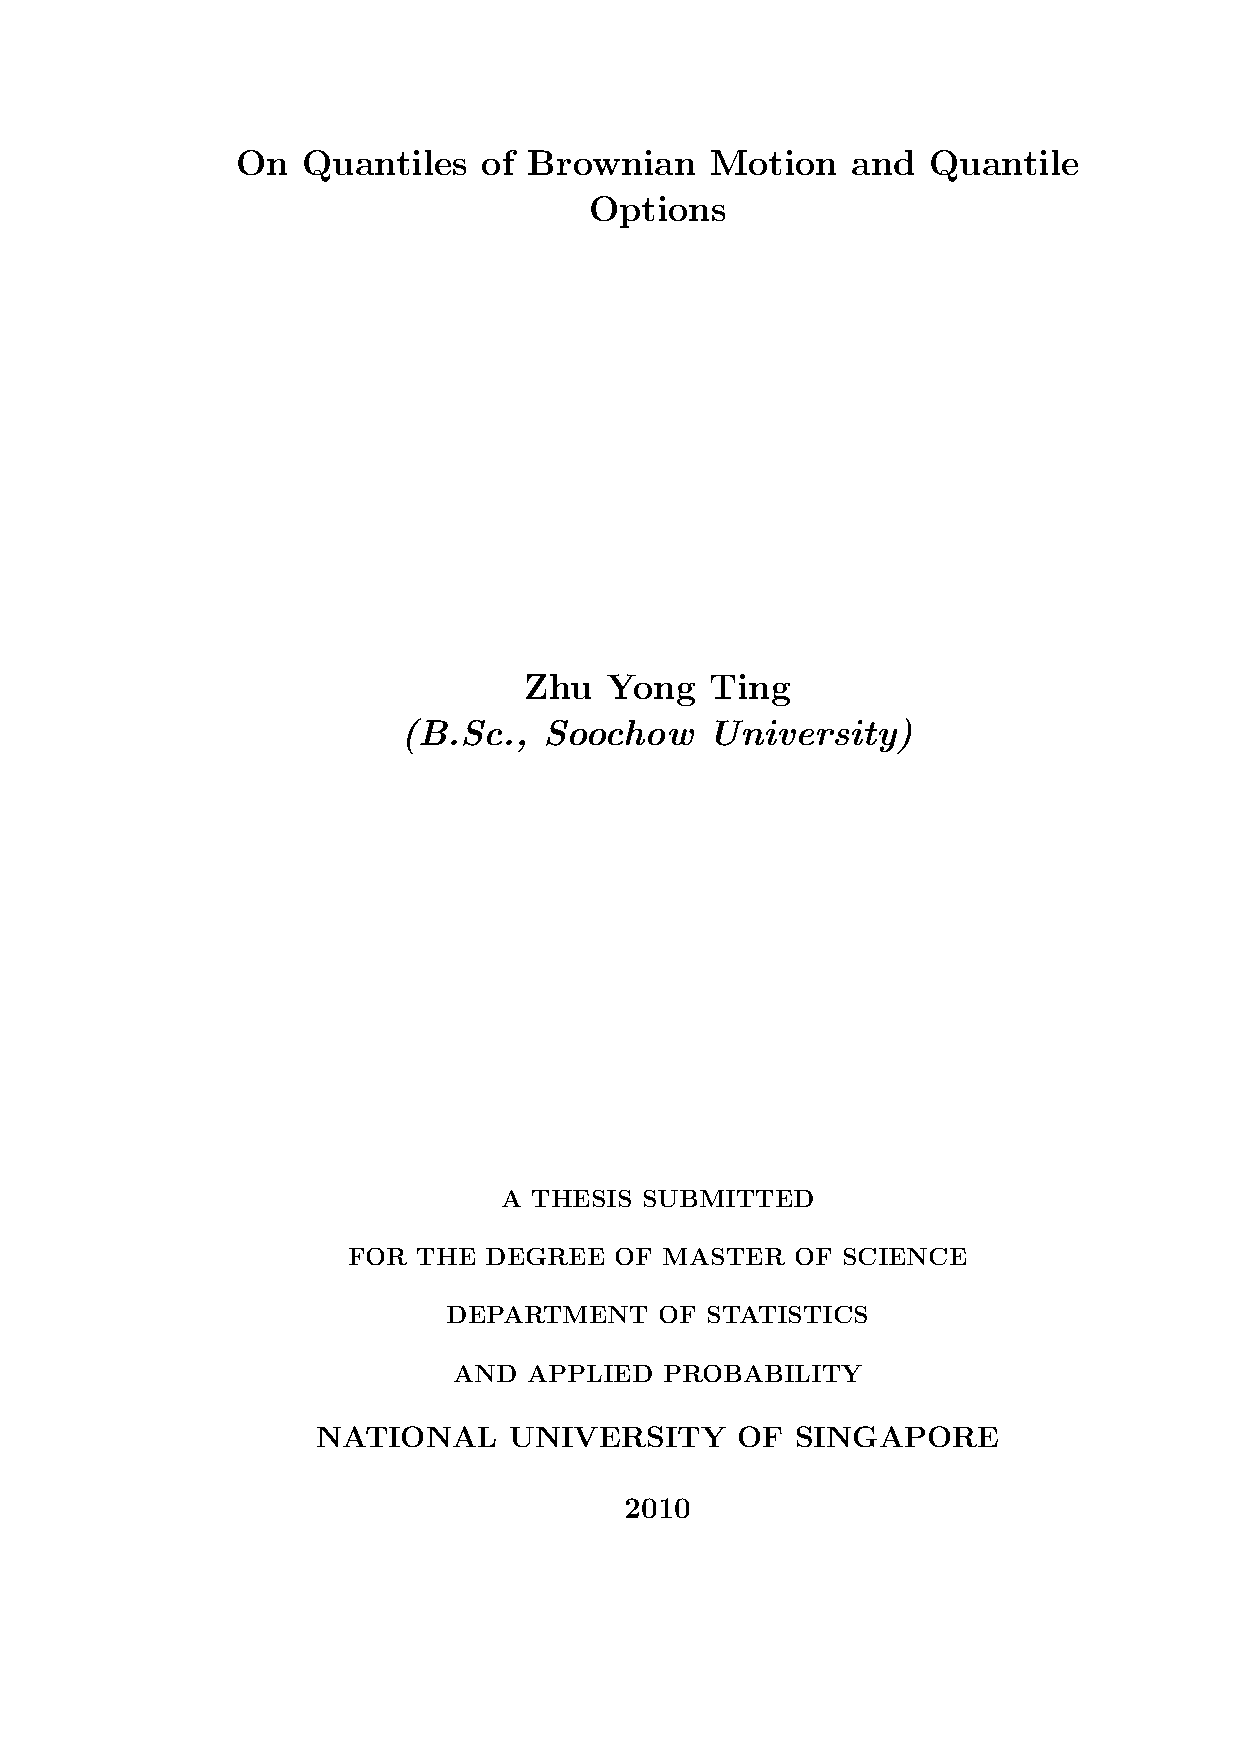
\includegraphics[]{notes.pdf}

Similarly, the value of the put is 
\begin{equation}
\begin{split}
LP_{fixed} =& -S_0 N(-d) + e^{-rT} KN(-d + \sigma \sqrt{T})  \\
&+ e^{-rT} \frac{\sigma^2}{2r} S_0 [ (\frac{S_0}{K}^{-\frac{2r}{\sigma^2}}N(-d+\frac{2r}{\sigma}) - e^{rT}N(-d)]
\end{split}
\end{equation}
if $K\leq S_0$, otherwise
\begin{equation}
\begin{split}
LP_{fixed} = & e^{-rT} (K-S_0) - S_0 N(-d) + e^{-rT}S_0 N (-d + \sigma \sqrt{T}) \\
&+ e{-rT} \frac{\sigma^2}{2r} S_0 [ N(-d + \frac{2r}{\sigma} \sqrt{T}) -e^{rT}N(-d)]
\end{split}
\end{equation}
 





As for American option, the complete solution should provide both the option value and an optimal exercise strategy. Due to this complicity, usually we need use numerical approach to solve the problem of pricing American style lookback option. In \cite{Lim2004}, for American \emph {fixed strike} lookback option they provide an full approach to compute the price and the optimal exercise boundary. In that paper, they first propose a space-time transformation which can reduce the valuation of a group of American lookback options to a single canonical optimal stopping problem for standard Brownian motion. Under this transformation, calendar time is scaled by square of volatility. Therefore, the canonical time horizon is only a small part of time to expiration. In addition, the transformation also removes the dependence on a prescribed root node which then make computing the entire early excise boundary by backward induction possible.

%Fix a process $X_t$, define $M_t = \max_{0\leq s\leq t} X_s$.
%When $X_t$ is a standard brownian motion without drift,
%the joint distribution of $M_t$ and $X_t$ can be easly calculated by reflection principle\cite{Karatzas91}:
%\[
%P(X_t \in a+dx, M_t \in b+dm) =
%\]

\chapter{Numerical Methods}

For American, and path-dependent options, generally closed form pricing formulaes are not available. In this case,usually numerical methods may be required. Even for Black Scholes formula, in practice, integration and the normal probability are obtained numerically. In this chapter, we provide a brief summary of the major numerical methods for option pricing. The most popular numerical approaches are lattice method, finite difference and Monte Carlo simulation. Generally speaking, different numerical methods are applicable in different situations. 
\subsection{Lattice Methods}
Lattice methods, also known as tree methods, use discrete time and discrete state approximations to the evolvements of underlying assets to calculate option prices. Lattice methods was originally proposed in
Cox, Ross, and Rubinstein 1979. Lattice approaches are popular because lattice methods are easy to understand and implement. In risk neutral valuation framework, as we discussed, the underlying price follows $S_{t+h} = S_t e^{Z}$, and $Z ~ N((r-\frac{1}{2} \sigma ^2)h,\sigma ^2 h)$. In lattice method, over a discrete time interval, one discrete random variable $X$ is used to approximate $Z$. $X$ takes value as $x_i$ with probability $p_i$ $i=1,2,...,m$. If $m=2$, it is binomial tree; If $m=3$, it is trinomial method. The value of the parameters of the distribution of the discrete random variable $X$ are chosen to approximate the distribution of continuous random variable $Z$ exactly or consistently. Under risk neutral method, the value of an option is the discounted present value of the expectation of the option's payoff. In lattice method we first use discrete diagram to approximate the continuous path of the price of underlying asset. Then calculate the discrete expectation of payoff as an approximation of option price. Due to the simplicity of lattice method, adjusted lattice methods for models with dividends, barriers and other complicated features can be easily constructed. However, the key issue of lattice method is the trade off between speed and accuracy. 




%\subsection{Finite Difference}
%Schwartz (1977) is the first to apply the finite difference
%technique to price options when closed form solutions are
%unavailable. Specially, he considered an American option on a stock
%which pays discrete dividends, which is quite common in real world.
%This method provides a practical numerical solution to the option
%pricing problem, and the optimal early exercise strategy as well.

%Unlike the ideal case in Black-Scholes model, in practice, we need
%to consider the valuation of an option which pays discrete dividends
%and also allow for early exercise (American-style option). In this
%case, the partial differential equation (PDE) which determines the
%value of the options is the same as in the Black-Scholes Model, but
%the boundary conditions will be different due to the early exercise
%feature and the payment of dividend. More specifically, let $f$
%represent the value of an American call option on a Stock with the
%price of $S$, and expires at time $T$. The PDE is (equivalent to
%equation (2.13))
%\begin{equation}
%\frac{\partial f}{\partial t}=rf-rS \frac{\partial f}{\partial S} -
%\frac{1}{2}\sigma^2 S^2\frac{\partial^2 f}{\partial S^2}
%\end{equation}
%subject to the boundary conditions:
%\begin{equation}
%\begin{split}
%& f(0,T)=0 \\
%& f(S,T)\rightarrow S, \text{ as } S\rightarrow \infty  \\
%& f(S,T)=\max(S-K,0)\\
%& f(S,T^+)=\max(0, S-K, f(S-D,T^-))
%\end{split}
%\end{equation}
%where $T^+$ and $T^-$ are the instants just before and just after
%the sock pays the discrete dividend $D$. The last condition reflects
%the fact that the stock price drops by $D$ as the dividend is paid,
%and indicates that it is optimal to exercise the option just before
%the dividend is paid whenever the value $S-K$ is greater than the
%option value $f(S-D,T^-)$ right after the dividend is paid.
%Unfortunately, the equation (2.20) with the boundary conditions (2.21) has no closed form solution, but can be solved numerically by approximating the partial derivatives with finite differences.

%We can estimate the derivative $\frac{\partial f}{\partial S}$ at



\subsection{Monte Carlo Simulation}



\chapter{$\alpha$-quantile}
For a stochastic prcess $X_t$,
the $\alpha$-quantile $( 0 \leq \alpha \leq 1)$
is defined by
\[
M(\alpha,t)(\omega) = \inf\Set{x:\int_0^t 1_{(X_s (\omega)\leq x)} > \alpha t}.
\]
Then we can see that $\inf_{0\leq s \leq t}  X_s = lim_{\alpha\to 0}M(\alpha,t)$ and $\sup_{(0\leq s \leq t})  X_s = lim_{\alpha\to 1} M(\alpha, t)$. In this sense $\alpha$-percentile option can be considered as a general class of lookback option. Unlike lookback option whose payoff depends on the maximum or minimum of the price of sock before maturity as mentioned before, $\alpha$-percentile option's payoff depends on the quantile of the stock price process. This option was first introduced by Miura\cite{Miura} in 1992. In 1995, Akahori\cite{Akahori1995} gave a generalized arc-sine law for this type of options by Feynman-Kac formula.
When $X_{t}$ is a Brownian motion $B_t$, using similar mathematical tools, Dassios obtained the explicit density of quantile option and gave a exceptional representation of the distribution of quantile.  In \cite{Dassios1995}, for $\alpha\in[0,1]$, $t\leq 0$, Dassios proved that
\begin{equation}\label{eq:Dassios}
M(\alpha, t) \eqlaw \sup_{s \leq \alpha t} X_s + \inf_{s\leq (1-\alpha)t} X'_s ,
\end{equation}
where $X'$ is a independent copy of $X$. Later in 1995, Embrechts, Rogers and Yor \cite{EmRoge1995} gave two proofs of this theorem without using Feynman-Kac computations.
\subsection{The advantage of $\alpha$-quantile option}
\cite{Ballotta2001}
\subsection{The distribution function of $\alpha$-quantile of Brownian motion}
In 1995, Yor gave the distribution function of the $\alpha$-quantile of Brownian motion without drift in \cite{Yor1995}. He obtained this result by simplifying related integral expressions on Miura \cite{Miura}. When $\mu = 0$, that is Brownian motion $B_t$ is without drift, define $\theta = ((1 - \alpha)/(\alpha))^{1/2}$, for the Brownian quantiles on time interval $[0, 1]$,  in \cite{Yor1995} we find:
\begin{equation}
P(M(\alpha,1)\in dx)= \begin{cases}
\sqrt{2 / \pi}exp(-x^2 / 2) \Phi(|x| / \theta)dx  &  \text{if } x \leq 0 \\
\sqrt{2 / \pi}exp(-x^2 / 2) \Phi(\theta x)dx  &  \text{if } x \geq 0
\end{cases}
\end{equation}
where
\begin{equation}\label{eq:density}
\Phi (x) = \sqrt{2/ \pi} \int^{\infty}_x dy exp(-y^2 / 2) = P (|N| \geq x)     (x \geq 0),
\end{equation}
with $N$ a standard Normal random variable.


When $u \neq 0$, Dassios  in \cite{Dassios1995} addressed this question for a more general case.  As stated in equation (\ref{eq:Dassios}), the density of


\subsection{Tree method for European Option}
Like lookback option, quantile option is also path-dependent. What makes things difficult is that quantile option is not markov. Normal tree methods which usually involve backward induction do not work in this case. We need to record all the information of the path because of lack of markov property, which will lead the tree to explosion computationally.
Kwok and Lau in \cite{Kwok2001} proposed a special way to apply tree method to price quantile option. In this paper, they find a relation between the price of quantile option and the price of cumulative Parisian option. By this approximation, they can simplify the pricing of quantile option. In their paper, they assume that there are $M$ time steps for the whole monitoring period $[0,T]$, and they define ${S^M}_j$, $j = - M$, ...$0$,$1$,...,$M$ as the discrete asset prices at maturity. Under trinomial tree method, the possible prices happened in one tree are limited to ${S^M}_j$,  $j = - M$, ...$0$,$1$, ...,$M$, which is also true for the value taken by quantile of brownian motion. Therefore they derived that
\begin{equation}\label{eq:kowk1}
V(\alpha, T) = e^{-rT} \sum^{M}_{j=-M}P[M(\alpha,T)=S^{M}_{j}]\max(S^{M}_{j}-X,0),
\end{equation}
where $V(\alpha,T)$ is for the value of $\alpha$-quantile option whose maturity it $T$, $P[M(\alpha,T)=S^{M}_{j}]$ is the probability that the quantile of Brownian motion achieve the value ${S^M}_j$,  $j = - M$, ...$0$,$1$, ...,$M$. In their paper, they observed that the difference between the prices of two cumulative Parisian binary options is a good approximation for $P[M(\alpha,T)=S^{M}_{j}]$ multiplies discount factor $e^{-rT}$, ie.
\begin{equation}\label{eq:kowk2}
e^{-rT}P[M(\alpha,T)=S^{M}_{j}] \approx V^{bin}_{cum}[(1-\alpha)T, S^{M}_{j-1}]-V_{cum}^{bin}[(1-\alpha)T, S_{j}^{M}]
\text{ for }j=-M, ... , 0, 1, ... , M
\end{equation}
where $V^{bin}_{cum}[d,B]$ is denoted as the price of continuously monitored cumulative Parisian binary option with down barrier $B$, and $d$ be the minimum cumulative time staying above the down barrier to avoid knock-out.


Combining equation (\ref{eq:kowk1})and (\ref{eq:kowk2}), they get
\begin{equation}\label{eq:kowk3}
V_{alp} = \sum^M_{j=-M} \max (S^M_j - X,0) \times \{V_{cum}^{bin}[(1-\alpha)T, S^M_{j-1}] - V^{bin}_{cum}[(1-\alpha)T, S^M_j]\} ,
\end{equation}
where $V^{bin}_{cum}[(1-\alpha)T, S_{-(M+1)}^M] = e^{-rT}$. By this result, we can turn pricing of quantile option into pricing of $2M+1$ cumulative Parisian option.


Parisian option is like an advanced version of barrier option. We know barrier option are options where the payoff depends on whether the underlying asset's price reaches a certain level (barrier) during the option's life. Barrier options usually trade in the over-the counter market. This kind of option is attractive because it is usually cheaper than similar option without barrier. Like vanilla option, barrier options also authorize holders the right to buy or sell, but  long sides of barrier options do not need to pay for scenarios they think is unlikely to happen in the future. One good example I find from wikipedia is about IBM. If you believe that IBM will go up this year, but are willing to bet that it won't go above \$100, then you can buy the barrier and pay less premium than the vanilla option. But in this one-touch knock-out or knock can bring difficulties to option writers when asset price is close to barrier. Particularly in the foreign exchange market where manipulation of underlying asset price is not impossible. To overcome short period price manipulation, various adjustments to one-touch knock out or knock in have been performed in practice. Parisian option is one solution.  In order to get activated, the underlying assets of parisian option need to stay in the knout out or knout in region for certain period of time. The payoff of a cumulative Parisian option is dependent on the total amount of time the underlying asset price has spent above or below barrier. As for binary option, the payoff is either some fixed amount of some asset or nothing at all.

\subsection{pricing cumulative parisian binary option by FSG}
Kwok and Lau also proposed a forward shorting grid(FSG) to price cumulative parisian option in \cite{Kwok2001}. The character of FSG is that this approach need add additional information at each node of  a lattice tree. Commonly in pricing path-dependent option, at each node we should add state vector to represent the path-dependent attribute, such as the extreme value of the underlying asset price achieved in lookback option case. As we know Hull and White \cite{Hull1993} and Ritchken, Sankarasubramanian and Vijh \cite{Vijh1993} were the first authors suggested this approach. In 1996, Barraquand and Pudet \cite{Barraquand1996} introduced a comprehensive framework for FSG. In this paper they indicated that the FSG method is unconditionally convergent. Further, they showed that when the covariance matrix is degenerate, the FSG method can outperform finite difference methods. The convergence of the FSG algorithm in pricing of Asian options was studied by Forsyth, Verzal and Zvan \cite{Forsyth1999}. Foesyth et al. pointed out that

 In Kwok and Lau's paper\cite{Kwok2001}, they constructed a trinomial tree to get the price of cumulative parisian option. But due to the fact that the result is not steady according to the setting of the length of up movement between each immediate steps, we modify their method to binomial tree.

In building binomial tree, we start by cutting the entire life of one option into many small time intervals of length $\Delta t = T / M$.
Our tree is build to mimic the the logarithm process of underlying asset price. Denote $x=\ln S$. In each step, the logarithm of the price of underlying asset is assumed to move from its initial value of $x_0$ to one of the two new values, $x_0 + d + u$ and $x_0 + d - u$ with equal probability,that is $p_{up} = p_{down} = 0.5$ , where $u = \sigma \sqrt{\Delta t}$ and $d = (r - {\sigma}^2 /2)\Delta t$. Here $\sigma$, and $r$ are volatility and riskless interest rate, respectively. The model is illustrated in Figure~\ref{fig:tree1}.
\begin{figure}[htbp]
   \centering
   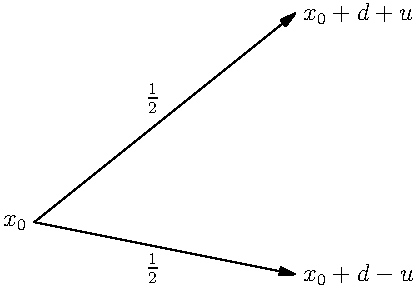
\includegraphics{trees.pdf} % requires the graphicx package
   \caption{Forward shooting}
   \label{fig:tree1}
\end{figure}

Like the notation used in \cite{Kwok2001}, we denote $V[m,j;k]$ as the numerical option value of the cumulative parisian option at the $m$-th time interval,  $j$ upward jumps from the initial underlying asset value and $k$ times breaches so far. Let $g(k,j)$ be the grid function that describes the correlated evolution of number of breaches $k$ and price indicate $j$. Denote $x_j$ be the value of $x$ corresponding to $j$ upward movements on the binomial tree. Then we should add $1$ to the indicator $k$ if the underlying asset price $S$ is no more than the barrier $B$; i.e $x_j \leq \ln B$. Hence we can see that a suitable setting of the grid evolution function $g(k,j)$ should be
\begin{equation}\label{eq:grid}
g(k,j) = k + 1_{\Set{x_j \leq B}}
\end{equation}
where $1_{\set{x_j \leq B}}$ is the indicator function. It is defined as
\begin{equation}\label{eq:grid-indicator}
1_{\Set{x_j \leq B}} =  \begin{cases}
1 & \text{if } x_j \leq \ln B \\
0 & \text{if } x_j > \ln B
\end{cases}
\end{equation}
Then the FSG method for pricing the cumulative Parisian binary option can be expressed as
\begin{equation}\label{eq:fsg}
V[m-1,j;k] =\set{0.5V[m,j+1;g(k,j+1)]+0.5V[m,j-1,g(k,j-1)]}e^{-r\Delta t}
\end{equation}
for $m-1 < M$.


Let $N$ be the predetermined number of breaches recored for the all duration of the life of an option that is desired to activate   the contract.
Considering the binary feature of the option, we should initiate our algorithm with
\begin{equation}\label{eq:initiate}
V[M,j;k] = \begin {cases}
1 & \text{if }  k < N \\
0 & \text{if }  k \geq N
\end{cases}
\end{equation}
By (\ref{eq:initiate})  (\ref{eq:fsg}) and backward induction, we can get the price of cumulative Parisian binary option with any prescribed times of breaches and barrier.

Recall what we get by equation (\ref{eq:kowk2}). In order to get the price of $\alpha$-quantile option, we can use the prices of $2M + 1$ cumulative Parisian binary options to approximate $\alpha$-quantile option's value. Hence using the FSG method we described above to calculate the prices of cumulative Parisian option  and doing a simple math work by equation (\ref{eq:kowk2}), we can get the approximated price for $\alpha$-quantile option with $M$ time steps.

Recall we defined earlier $\Delta t = T / M$. We compute the approximated option price of an $\alpha$-quantile call option with different time steps using equation (\ref{eq:kowk2}). As you can see in Figure % add figure ,
the numerical values of option are plotted against varying $\Delta t$. The values of parameters of the $\alpha$-quantile call option are set as: $ \alpha = 0.8$, $S_0 = 100$, $X = 95$, $r = 5\%$, $\sigma = 20\%$, and $T = 0.25$.
\begin{figure}[htbp]
   \centering
   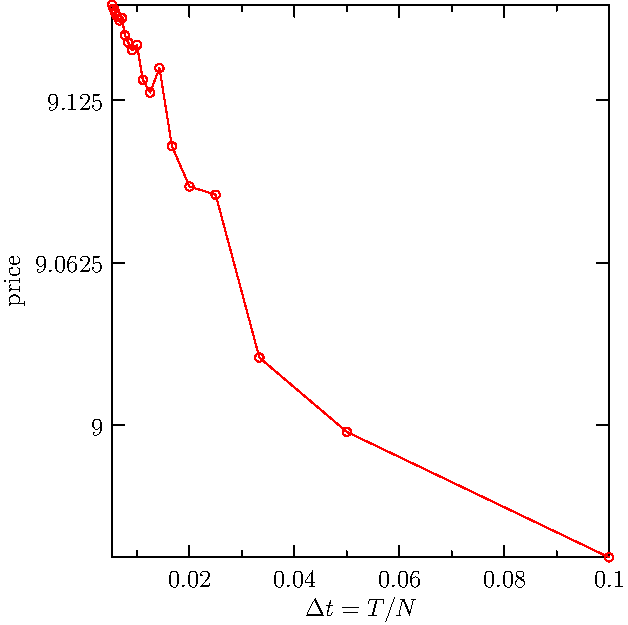
\includegraphics{bfsg.pdf} % requires the graphicx package
   \caption{example caption}
   \label{fig:2}
\end{figure}


\subsection{ an exponential time tree for American $\alpha$-quantile option}
% to be add













\section{Discrite v.s. continous}
\subsection{Euler scheme and randon walk}
approximate brownian by random walk through Euler scheme.


\subsection{path transform}
Let $S_k$ be a randon walk (assume $S_0=0$)
with i.i.d increasment, i.e.
$\Delta S_k = S_k -  S_{k-1}$ is i.i.d.
Define the ordered statistics $M_{k,n}$ be the $k$th-smallest value in
$\Set{S_i}_{i=0}^n$.
Under this setting, clearly, $M_{0,n} = \inf_{0\leq i\leq n}S_i$
and $M_{n,n} = \sup_{0\leq i\leq n}S_i$
Define
\[S'_i = S_{i+k}-S_k\]
for fixed $k, n$.

In Wendel's paper\cite{Wendel1960}, an identity about randon walk with
i.i.d increasment was dirived:
\begin{equation}\label{eq:dpathdec}
(M_{k,n}, S_n) \eqlaw (\sup_{i\leq k} S_i +\inf_{i\leq n-k} S'_i, S_n)
\end{equation}

In
\cite{Chaumont1999}, Chaumont provide a combinatorics treatment.
He constructed a explicit path transform for $S$ to $\tS$, such that
\[
(M_{k,n}, S_n) = (\sup_{i\leq k} \tS_i+\inf_{i\leq n-k} \tS'_i, \tS_n)
\]
Here $\tS$ has same distribution with $S$ and each path $S$
 one-one corresponed to $\tS$.

By using path transform, Chaumont proved
following continous version of path decomposition:
\begin{equation}\label{eq:cpathdec}
(M_{\alpha,T}, S_T) \eqlaw (\sup_{t\leq \alpha{T}} S_T +\inf_{t \leq (1-\alpha)T} S'_t, S_T)
\end{equation}
where as above:
\[
S'_t = S_{\alpha T+t} - S_{\alpha_T}.
\]

For Brownian motion case, this formular were proved in many differet ways
and original due to Dassios\cite{Dassios1995}.

\subsection{an estimate of week discrete error}
\cite{Janssen2008} gives a estimate of the difference of  expatations
between maximum of borwnian motion and associated random walk.
Since we just give a really rough estimate, we only list the first two term.
For $B_t$ a Borwnian motion with drift $\mu$ and variance $1$ on time interval $[0,1]$, that is $B_t = \mu t + W_t$, where $W_t$ is standard Brownian motion, we can get
\begin{equation}\label{eq:est1}
E\max_{0\leq t \leq 1} B(t) - E\max_{n=0,\cdots, N}B(n/N)
= -\frac{\zeta(1/2)}{\sqrt{2\pi N}}-\frac{2g(1)-\mu}{4N} + O(1/N^{3/2})
\end{equation}
where
\[
g(t) = \mu \Phi(\mu \sqrt{t}) + \frac{1}{\sqrt{2\pi t}} e^{-\frac{1}{2}\mu^2 t}.
\]
\[
\zeta(1/2) \approx -3.92264613.
\]

For general Borwnian $\tB(t)$ motion on time interval $[0,T]$ with drift $\tmu$, variance $\tsigma$,
we use following transform
\begin{align*}
\tB_t &= \tsigma \sqrt{T} B_{t/T} = \tsigma \sqrt{T} \mu t/T
+ \sqrt{T}\tsigma W_{t/T}\\
\mu &= \tmu \sqrt{T}/\tsigma
\end{align*}
do derive the follwoing formula:
\begin{equation}\label{eq:maxest}
E\max_{0\leq t\leq T} \tB(t) - E \max_{0\leq n \leq N} \tB(nT/N) =
 -\frac{\zeta(1/2)}{\sqrt{2\pi}}\tsigma \sqrt{T/N}
 -\frac{2g(1)-\tmu\sqrt{T} / \tsigma}{4N}\tsigma\sqrt{T} +
O(\sqrt{T}/N^{3/2})
\end{equation}

Now combine $(\ref{eq:cpathdec})$ $(\ref{eq:dpathdec})$ and $(\ref{eq:maxest})$, for $0 < \alpha < 1$,
we get an very rough estimate of the apporximation order:
\begin{equation}
\begin{split}
\E (M_{\alpha,T}) - \E (M_{k,N})
=& \EE{\sup_{t\leq \alpha{T}} S_t +\inf_{t \leq (1-\alpha)T}S'_t}
- \EE{\sup_{i\leq k} S_i+\inf_{i\leq N-k} S'_i}\\
=& \EE{\sup_{t\leq \alpha{T}} S_t +\inf_{t \leq (1-\alpha)T}S'_t
-  \sup_{i\leq k} S_i-\inf_{i\leq N-k} S'_i} \\
= &  \EE{\sup_{t\leq \alpha{T}} S_t - \sup_{i\leq k} S_i} +
\EE{\inf_{t \leq (1-\alpha)T} S'_t-\inf_{i\leq N-k} S'_i}\\
=& -\frac{\zeta(1/2) \tsigma}{\sqrt{2\pi}}\left(\sqrt{T/\alpha N}
\sqrt{\alpha} - \sqrt{T/(1-\alpha)N}\sqrt{1-\alpha}\right) \\
& - \frac{2g(1)}{4}\sqrt{T} \tsigma
\left(\frac{1}{\alpha N} \sqrt{\alpha}
  - \frac{1}{(1-\alpha)N}\sqrt{1-\alpha}\right) \\
& + \tmu \left( \frac{1}{4\alpha N}\alpha
  +\frac{1}{4(1-\alpha)N}(1-\alpha)\right)T
+ O(\sqrt{T}/N^{\frac{3}{2}}) \\
=& - \frac{2g(1)\sqrt{T}\tsigma}{4N}
\left(\frac{1}{\sqrt{\alpha}}
  - \frac{1}{\sqrt{1-\alpha}}\right) \\
& + \frac{\tmu T}{2 N}
+ O(1/N^{\frac{3}{2}})
\end{split}
\end{equation}
where $k = \alpha N$.
The second last equality holds by view $\inf_{t\leq (1-\alpha)T} S'_t$ as
$-\max_{t\leq (1-\alpha)T} (-S'_t)$.

This estimate shows that the convergence order
are all $\frac{1}{2}$ when $\alpha \neq 1/2$. If $\alpha=1/2$ and the
Brownian motion does not have  drift ($\mu=0$), it is easy to see
(by noting that
$\E M_{1/2,T} = \E -M_{1/2,T}$) $\E M_{1/2,T} = \E M_{k,n} = 0$.
When the Brownian motion has drift, the order becomes $1$.

Now, suppose that $f$ is an monotone Lipschitz continous function.
WLOG, asuume
\begin{equation}\label{eq:lips}
0 \leq f(x)-f(y) \leq C (x-y) \quad \forall x>y,
\end{equation}
where some counstant $C$. This aways the case when $f$ the
(truncated) payoff of a $\alpha$-quantile option.

Then it is easy to see
\[
-C\left( \sup_{i\leq n-k} (-S'_i)-\sup_{i\leq n-k} (-S'_i)\right)
 \leq f(M_{\alpha,T}) - f(M_{k,N})
\leq  C \left(\sup_{t\leq \alpha{T}} S_t - \sup_{i\leq k} S_i\right)
\]
Hence
\[
\abs{\E f(M_{\alpha,T}) - \E f(M_{k,N})}
\leq \max\Set{\sqrt{\alpha}, \sqrt{1-\alpha}}
C\frac{-\zeta(1/2)}{\sqrt{2\pi}}\sqrt{T/N}  + O(1/N)
\]


\subsection{a study of the joint distribution of Brownian motion and its $\alpha$-quantile}
In this section we are going to provide a give the joint distribution of Brownian motion and its quantile. When the Brownian motion is without drift,
ie $\mu = 0 $,
As we know the joint distribution of runing maximal and end point of
standard Brownian motion at time $\tau$ is
\[
P(X_\tau\in da, M_\tau\in db) =
\frac{2(2b-a)}{\sqrt{2\pi \tau^3}} \exp(-\frac{(2b-a)^2}{2\tau})
I_{\Set{a\leq b, b\geq 0}} (a,b) da db \triangleq p_\tau(a,b)
\]

To deal with the distribution of $\alpha$-quantile, we usetwo copy of
Brownian motion and denote corresponding value at
$\tau=\alpha t$(respectively $\tau=(1-\alpha) t$) by $X_1$(resp. $X_2$) and
maxiamal $M_1$(resp. $M_2$).
Then
\[
\begin{split}
(X_1,M_1, X_2, M_2) \sim& P(X_1\in dx_1, M_1\in dm_1, X_2\in dx_2, M_2\in dm_2)\\
&= P_{\alpha t}(x_1, m_1) P_{(1-\alpha)t}(x_2,m_2) dx_1dm_1dx_2dm_2
\end{split}
\]


Use the transform
\[
\begin{pmatrix}
X_1\\ X_2\\ M_1\\ M_2\\
\end{pmatrix}
\overset{
\begin{pmatrix}
1 & 1 & 0 &0 \\
1 & -1 & 0 & 0 \\
0 & 0 & 1 & 1\\
0 & 0 & 1 & -1\\
\end{pmatrix}
}{\longrightarrow}
\begin{pmatrix}
X_1+X_2\\
X_1 - X_2 \\
M_1 + M_2 \\
M_1 - M_2 \\
\end{pmatrix}
\triangleq
\begin{pmatrix}
X \\ \tX\\ \tM \\M
\end{pmatrix}
\]

And
\[
(X, \tX, M, \tM) \sim \frac{1}{4} P_{\alpha t}(\frac{x+\tx}{2},\frac{m+\tm}{2})
P_{(1-\alpha)t}(\frac{x-\tx}{2},\frac{\tm-m}{2}) I_D,
\]
where $D$ is the domain $\Set{x_1\leq m_1, x_2\leq m_2, m_1 >0, m_2>0}$


Hence (use change of variable $x' = (x+\tx)/2$ and $m' = (m+\tm)/2$
\[
\begin{split}
&P(M_{\alpha,t}\in dm, X_t \in dx) = P(M_1-M_2\in dm, X_1+X_2\in dx) \\
=& \frac{1}{4} \int_{-\infty}^{\infty}\int_{-\infty}^\infty
P_{\alpha t}(\frac{x+\tx}{2},\frac{m+\tm}{2})
P_{(1-\alpha)t}(\frac{x-\tx}{2},\frac{\tm-m}{2}) I_D d\tx d\tm\\
= & \int_{-\infty}^{\infty}\int_{-\infty}^\infty
P_{\alpha t}(x',m')
P_{(1-\alpha)t}(x-x',m-m') I_{D'} d\tx d\tm\\
= & \int_{\max\Set{0,m}}^{\infty} \int_{x+m-m'}^{m'}
P_{\alpha t}(x', m') P_{(1-\alpha)t}(x-x',m'-m) dx' dm',
\end{split}
\]
where domain $D' = \Set{x' \leq m', x-x'\leq m'-m, m'>0, m'-m>0}$.


\bibliography{prob}

\end{document}  